\chapter{牛顿运动定律}\label{ch:b1:newton-dynamics}

一名跳伞者跳出机舱，不到十几秒便不再加速：
速度达到每小时二百千米时，空气向上的阻力恰好与地球的引力相等。
汽车转弯过快，轮胎便会打滑；
山路上的卡车以低挡位缓慢爬行，
靠的正是让它在平路上能够停住的同一种摩擦力。运动学描述运动，
动力学则解释运动，其依据是一条
把物体的加速度与作用于它的力联系起来的定律。本章
叙述牛顿三大定律，归纳本册所涉及的各种力：
重力、弹簧力、绳的张力、接触力，以及干摩擦与流体阻力，
并说明如何从受力图出发，
得到一个微分方程及其解。

\begin{omfigure}
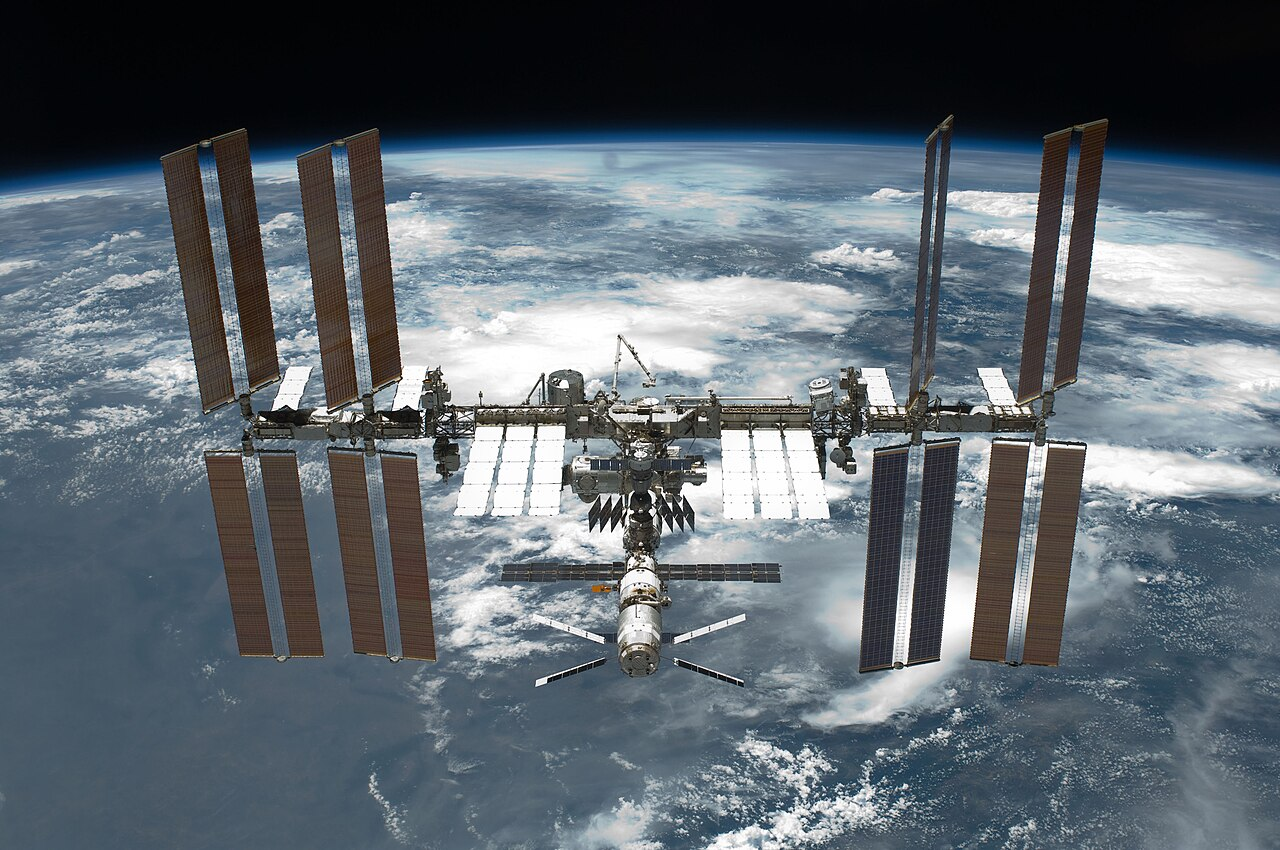
\includegraphics[width=0.60\linewidth]{images/book3/iss-orbit.jpg}

{\small 从离开的航天飞机上所见的国际空间站（NASA）：站内一切物体共同处于自由落体状态，这正是站内物体看似没有重量的原因。}
\end{omfigure}

\section{质量、动量与三大定律}

\begin{definition}[质量、动量、力]\label{def:b1:newton-dynamics:momentum}
\index{质量}\index{动量}\index{力}
质点具有\emph{惯性质量}$m > 0$（单位为千克），
它是质点抵抗速度变化的量度，与参考系无关。
质点在某参考系中的\emph{动量}为
\[
\vect p = m\,\vect v \qquad (\unit{kg.m/s}).
\]
\emph{力}$\vect F$（单位为牛顿）是另一物体对质点的作用；
力按矢量相加，\emph{合力}即其和
$\sum\vect F$。
\end{definition}

\begin{theorem}[牛顿定律]\label{thm:b1:newton-dynamics:laws}
\index{牛顿定律}\index{惯性参考系}\index{惯性原理}\index{作用与反作用}
\begin{enumerate}
  \item \emph{惯性原理。} 存在一类参考系，称为
        \emph{惯性}（或伽利略）参考系，在其中，
        不受力或合力为零的质点，沿直线
        以恒定速度运动。与惯性参考系做匀速直线平动的任一参考系，
        亦为惯性参考系。
  \item \emph{动量定律。} 在惯性参考系中，
        \[
        \frac{\dd\vect p}{\dd t} = \sum\vect F, \qquad \text{即}\qquad
        m\,\vect a = \sum\vect F \ \text{ 对常量 } m .
        \]
  \item \emph{作用与反作用。} 若物体 $A$ 施力 $\vect F_{A\to B}$
        于物体 $B$，则 $B$ 施力 $\vect F_{B\to A} = -\vect F_{A\to B}$
        于 $A$，沿二者连线方向。
\end{enumerate}
\end{theorem}
\admitted

\begin{remark}[定律的含义]\label{rem:b1:newton-dynamics:meaning}
第一定律并非第二定律的特例：它\emph{规定}了
第二定律成立的参考系。实际上，对于持续数分钟的实验，
地球上的实验室可视为惯性系，精度极高（误差见
\cref{ch:b1:non-inertial-frames}）；与太阳及遥远恒星相固连的参考系则更为精确。
第二定律是一个矢量方程，等价于三个标量方程，每个坐标轴一个，
选取坐标轴（见\cref{ch:b1:point-kinematics}）
是每个问题的第一步决定。
第三定律在本册所涉及的接触力与引力中，
每一时刻都成立。
\end{remark}

\begin{definition}[封闭系统；动量守恒]\label{def:b1:newton-dynamics:conservation}
\index{封闭系统}\index{动量守恒}
\emph{封闭系统}与外界不交换物质。对于
质点系，内力两两相消（第三定律），
系统的总动量 $\vect P = \sum m_i\vect v_i$ 满足
$\dd\vect P/\dd t = \sum\vect F_{\mathrm{ext}}$：当外力为零时，
总动量守恒（在\cref{ch:b1:systems-of-points}中
对此作了展开）。
\end{definition}

\section{常见的力}

\begin{proposition}[重力与万有引力]\label{prop:b1:newton-dynamics:weight}
\index{重力}\index{引力场}
在地球表面附近，质量为 $m$ 的物体
受到其\emph{重力} $\vect P = m\vect g$ 的作用，其中 $\vect g$ 为当地的
引力场，$g \approx \qty{9.81}{m/s^2}$，方向竖直向下（近似指向
地心）。更一般地，质量为 $M$ 的物体在距离 $r$ 处吸引质量 $m$，
引力为 $\vect F = -GMm/r^2\,\vect e_r$（见\cref{ch:b1:central-forces}）；
在半径为 $R$ 的球面上，$g = GM/R^2$。注意单位：
\unit{N/kg} 与 \unit{m/s^2} 相同，这正是一切物体
下落情况一致的原因。
\end{proposition}

\begin{proof}
牛顿万有引力定律在本阶段不加证明地承认，并在
\cref{ch:b1:central-forces}中探讨；$g = GM/R^2 = 6.67\times10^{-11} \times
5.97\times10^{24}/(6.37\times10^6)^2 = \qty{9.8}{m/s^2}$。
\end{proof}

\begin{proposition}[弹簧；绳]\label{prop:b1:newton-dynamics:springstring}
\index{胡克定律}\index{弹簧}\index{张力}
劲度系数为 $k$、自然长度为 $\ell_0$ 的理想弹簧，被拉伸
至长度 $\ell$，沿从其固定端指向物体的单位矢量 $\vect u$ 方向，
对物体施加\emph{回复力}
\[
\vect F = -k(\ell - \ell_0)\,\vect u \qquad (\text{胡克定律}),
\]
指向其自然长度。理想绳（无质量、不可伸长）
沿绳方向施加\emph{张力} $\vect T$，即拉力，
两端及沿绳各处大小相同（即使绕过无质量、
无摩擦的滑轮）。
\end{proposition}

\begin{proof}
胡克定律是适用于小形变的经验模型。
对绳而言，无质量的绳元满足 $0 = \vect T_1 + \vect T_2$，
由牛顿第二定律可得，故张力不变地传递。
\end{proof}

\begin{proposition}[接触力：法向力与干摩擦]\label{prop:b1:newton-dynamics:friction}
\index{法向力}\index{干摩擦}\index{库仑摩擦定律}\index{摩擦因数}
与之接触的固体表面对物体施加\emph{法向力}
$\vect N$，垂直于表面且为排斥力（$N \geq 0$：表面
不能拉物体），以及切向的\emph{摩擦力} $\vect T$。
库仑摩擦定律：若物体不滑动，则 $\abs{\vect T} \leq \mu_s N$，
（\emph{静}摩擦力随所需而调整，直至该极限）；
若物体以相对表面的速度 $\vect v_g$ 滑动，
$\vect T = -\mu_d N\,\vect v_g/\abs{\vect v_g}$（\emph{动}摩擦力，
与滑动方向相反），其中 $\mu_d \leq \mu_s$ 为摩擦因数，
数量级约为 $0.1$ 到 $1$，取决于材料，与接触
面积及速率无关。
\end{proposition}
\admitted

\begin{omfigure}
\begin{tikzpicture}[font=\small, x=1cm, y=1cm]
  % incline
  \draw[thick] (0,0) -- (6,0) -- (0,3.0) -- cycle;
  \node at (4.8,0.32) {$\alpha$};
  \draw (6,0) ++(-1.2,0) arc (180:153.4:1.2);
  % block center on incline at x=3: surface point (3,1.5); normal direction (0.447,0.894) ; block square rotated 26.6 deg, approximate with a rotated rectangle
  \begin{scope}[shift={(3,1.5)}, rotate=-26.6]
    \draw[thick, fill=omDef!15] (-0.5,0) rectangle (0.5,0.7);
    \coordinate (G) at (0,0.35);
  \end{scope}
  \fill (G) circle (1.4pt);
  \draw[-Stealth, omThm, very thick] (G) -- ++(0,-1.6) node[below] {$m\vect g$};
  \draw[-Stealth, omDef, very thick] (G) -- ++(0.447*1.43,0.894*1.43) node[above right] {$\vect N$};
  \draw[-Stealth, omProp, very thick] (G) -- ++(-0.894*0.9,0.447*0.9) node[left] {$\vect T$};
  \draw[-Stealth] (5.0,2.2) -- ++(0.894*0.9,-0.447*0.9) node[right] {$x$};
  \draw[-Stealth] (5.0,2.2) -- ++(0.447*0.9,0.894*0.9) node[above] {$y$};
\end{tikzpicture}\qquad
\begin{tikzpicture}
\begin{axis}[omaxis, width=6.6cm, height=4.6cm, xlabel={施加力 $F$}, ylabel={摩擦力 $T$},
    xmin=0, xmax=3.2, ymin=0, ymax=2.2, xtick={1.5}, xticklabels={$\mu_sN$}, ytick={1.2,1.5}, yticklabels={$\mu_dN$,$\mu_sN$}]
  \addplot[omDef, thick, domain=0:1.5, samples=2] {x};
  \addplot[omThm, thick, domain=1.5:3.2, samples=2] {1.2};
  \draw[dashed, omExo] (axis cs:1.5,0) -- (axis cs:1.5,1.5);
  \node[omDef, font=\footnotesize, anchor=west] at (axis cs:0.15,1.75) {静止：$T = F$};
  \node[omThm, font=\footnotesize, above] at (axis cs:2.4,1.2) {滑动：$T = \mu_dN$};
\end{axis}
\end{tikzpicture}

{\small 左：斜面上物块所受的力——重力、法向力、
沿斜面的摩擦力——以及自然坐标轴。右：
库仑摩擦定律：静止时，摩擦力与施加的力平衡，直至
$\mu_sN$；一旦开始滑动，摩擦力降至 $\mu_dN$ 并保持于此。}
\end{omfigure}

\begin{proposition}[流体摩擦]\label{prop:b1:newton-dynamics:drag}
\index{流体摩擦}\index{阻力}\index{斯托克斯定律}
物体以速度 $\vect v$ 在静止流体中运动时，受到
\emph{阻力}，方向与 $\vect v$ 相反：低速（尺寸小、流体黏性大）时，
此时为线性，$\vect F = -\alpha\vect v$——对半径为 $r$ 的球，
在黏度为 $\eta$ 的流体中，$\alpha = 6\pi\eta r$（斯托克斯）；
高速（大而快的物体在空气或水中）时，
为二次的，
\[
\vect F = -\tfrac12\,\rho\,C_xS\,v\,\vect v ,
\]
其中 $\rho$ 为流体密度，$S$ 为物体迎流的截面，
$C_x$ 为无量纲的\emph{阻力系数}（球体 $0.5$，
汽车 $0.3$，平板圆盘 $1$）。雷诺数
$\rho vL/\eta$（见\cref{rem:b1:units-dimensions:pi}）决定：低于 $1$ 时为线性，
高于约 $1000$ 时为二次的。
\end{proposition}
\admitted

\begin{remark}[其他力]\label{rem:b1:newton-dynamics:others}
浮力（阿基米德）是压力的合力，在
\cref{ch:b1:fluid-statics}中推导；作用于电荷的电力与磁力
是\cref{ch:b1:charged-particles}的内容。本章所有的
力都是接触或场相互作用的\emph{模型}，
仅在规定范围内成立——胡克定律在弹簧断裂时失效，
库仑摩擦定律在高压下失效，斯托克斯阻力在高
速时失效。检验所用模型是否适用，是每个解答的一部分。
\end{remark}

\section{动力学问题的求解}

\begin{method}[从情境到方程]\label{met:b1:newton-dynamics:method}
\begin{enumerate}
  \item \emph{系统}：指定视为质点的物体。
  \item \emph{参考系}：指定参考系，并检验它是否为惯性参考系（或在所需精度内
        视作惯性系）。
  \item \emph{受力}：列出所有与系统接触或吸引系统的物体，
        并在受力图（隔离体图）上画出每个力；
        此外不计入其他任何因素。
  \item \emph{坐标}：选取适应运动的坐标轴
        （见\cref{met:b1:point-kinematics:choose}），并写出 $\vect a$。
  \item \emph{投影}：将 $m\vect a = \sum\vect F$ 投影到各坐标轴上，并利用
        约束条件（在表面上的物体始终留在表面上：$a_\perp = 0$；
        长度固定的绳：两端速率相等）。
  \item \emph{求解}并\emph{检验}：量纲、极限情况、
        正负号（$N \geq 0$，静止时 $\abs T \leq \mu_sN$）。
\end{enumerate}
\end{method}

\begin{example}[斜面上的物块]\label{ex:b1:newton-dynamics:incline}
质量为 $m$ 的物块位于倾角为 $\alpha$ 的斜面上，静、动摩擦因数分别为 $\mu_s$，
$\mu_d$。取坐标轴：$x$ 沿斜面向下，$y$ 沿法线方向。重力
$(mg\sin\alpha, -mg\cos\alpha)$，法向力 $(0, N)$，摩擦力 $(-T, 0)$（若下滑）。
沿 $y$ 方向：$N = mg\cos\alpha$。沿 $x$ 方向静止时：
$T = mg\sin\alpha \leq \mu_sN = \mu_smg\cos\alpha$，即 $\tan\alpha
\leq \mu_s$：物块静止的最大倾角为 $\arctan\mu_s$——
无需平衡即可测量 $\mu_s$ 的方法。滑动时：$ma = mg\sin\alpha -
\mu_dmg\cos\alpha$，于是 $a = g(\sin\alpha - \mu_d\cos\alpha)$，与 $m$ 无关，
当 $\alpha = 30^\circ$、$\mu_d = 0.2$ 时为 \qty{3.2}{m/s^2}。
\end{example}

\begin{example}[单摆]\label{ex:b1:newton-dynamics:pendulum}
\index{单摆}
质量为 $m$ 的小球系于长为 $\ell$ 的细绳上，细绳与竖直向下方向的夹角为 $\theta$。
悬点处取极坐标，$\vect a =
-\ell\dot\theta^2\,\vect e_r + \ell\ddot\theta\,\vect e_\theta$；受力为
重力 $mg(\cos\theta\,\vect e_r - \sin\theta\,\vect e_\theta)$ 与
张力 $-T\vect e_r$。沿 $\vect e_\theta$ 方向：$m\ell\ddot\theta =
-mg\sin\theta$，
\[
\ddot\theta + \frac{g}{\ell}\sin\theta = 0 ,
\]
当角度很小（$\sin\theta \approx \theta$）时，上式即为谐振动方程，
其中 $\omega_0 = \sqrt{g/\ell}$，周期 $T_0 = 2\pi\sqrt{\ell/g}$，
这里的 $k = 2\pi$ 正是 \cref{ex:b1:units-dimensions:pendulum} 所未能给出的。
沿 $\vect e_r$ 方向：$T = mg\cos\theta + m\ell\dot\theta^2$——
细绳在最低点拉力最大，此处速率也最大。
\end{example}

\begin{omfigure}
\begin{tikzpicture}[font=\small, x=1cm, y=1cm]
  \draw[thick] (-1,3.2) -- (1,3.2); \fill[pattern=north east lines] (-1,3.2) rectangle (1,3.45);
  \fill (0,3.2) circle (1.2pt);
  \draw[dashed] (0,3.2) -- (0,0.2);
  \coordinate (M) at ($(0,3.2)+(-65:2.8)$);
  \draw[thick] (0,3.2) -- (M);
  \fill[omDef] (M) circle (3pt); \node[below right] at (M) {$m$};
  \draw (0,2.3) arc (-90:-65:0.9); \node at (0.25,2.05) {$\theta$};
  \draw[-Stealth, omThm, very thick] (M) -- ++(0,-1.3) node[below] {$m\vect g$};
  \draw[-Stealth, omDef, very thick] (M) -- ++(115:1.6) node[pos=0.55, left, xshift=-2pt] {$\vect T$};
  \draw[-Stealth, omProp, thick] (M) -- ++(-65:0.9) node[right] {$\vect e_r$};
  \draw[-Stealth, omProp, thick] (M) -- ++(25:0.9) node[right] {$\vect e_\theta$};
  \draw[omDef!40] ($(0,3.2)+(-110:2.8)$) arc (-110:-60:2.8);
\end{tikzpicture}\qquad
\begin{tikzpicture}
\begin{axis}[omaxis, axis x line=bottom, width=7.2cm, height=4.8cm, xlabel={$t/\tau$}, ylabel={$v/v_\infty$},
    xmin=0, xmax=5, ymin=0, ymax=1.2, ytick={0.5,1}, xtick={1,2,3,4,5}]
  \addplot[omDef, thick, domain=0:5, samples=100] {1 - exp(-x)};
  \addplot[omThm, thick, domain=0:5, samples=100] {tanh(x)};
  \addplot[omExo, dashed, domain=0:5, samples=2] {1};
  \node[omDef, font=\footnotesize] at (axis cs:3.6,0.8) {线性阻力};
  \node[omThm, font=\footnotesize] at (axis cs:1.2,1.1) {二次阻力};
\end{axis}
\end{tikzpicture}

{\small 左图：单摆、它所受的两个力，以及用来投影牛顿定律的极坐标基；
右图：物体自静止下落，受重力与阻力作用，速率趋近终端
速度 $v_\infty$：线性阻力时按指数规律趋近，
其时间尺度 $\tau = m/\alpha$；二次阻力时为双曲正切，
其时间尺度 $\tau = v_\infty/g$。}
\end{omfigure}

\begin{proposition}[有阻力的下落；终端速度]\label{prop:b1:newton-dynamics:terminal}
\index{终端速度}
质量为 $m$ 的物体自静止下落，受重力与阻力作用，
最终达到两力平衡时的\emph{终端速度}。线性阻力情形：
$m\dot v = mg - \alpha v$，$v = v_\infty(1 - \eu^{-t/\tau})$，其中
$v_\infty = mg/\alpha$，$\tau = m/\alpha$。二次阻力情形：$m\dot v = mg -
\tfrac12\rho C_xSv^2$，$v = v_\infty\tanh(t/\tau)$，其中
\[
v_\infty = \sqrt{\frac{2mg}{\rho C_xS}}, \qquad \tau = \frac{v_\infty}{g} .
\]
\end{proposition}

\begin{proof}
线性情形为一阶方程，$\tau\dot v + v = v_\infty$
（见\cref{thm:b1:transient-regimes:firstorder}）。二次情形中，令
$u = v/v_\infty$，$\dot u = (1 - u^2)/\tau$；分离变量，
$\int\dd u/(1 - u^2) = \operatorname{artanh}u = t/\tau$（其中有理
分式 $1/(1 - u^2) = \tfrac12[1/(1 - u) + 1/(1 + u)]$ 的积分为
$\tfrac12\ln\frac{1 + u}{1 - u}$），于是 $u = \tanh(t/\tau)$。
\end{proof}

\begin{example}[两种终端速度]\label{ex:b1:newton-dynamics:terminal}
一名跳伞者，$m = \qty{80}{kg}$，俯卧姿势，$C_xS \approx \qty{0.8}{m^2}$
在空气中（$\rho = \qty{1.2}{kg/m^3}$）：$v_\infty = \sqrt{2 \times 785/(1.2
\times 0.8)} = \qty{40}{m/s}$，达到（至 $90\%$）所需时间约为 $1.5\tau =
\qty{6}{s}$。一颗雾滴，$r = \qty{10}{\micro m}$，处于斯托克斯区
（$\eta_{\text{空气}} = \qty{1.8e-5}{Pa.s}$）：$v_\infty = mg/6\pi\eta r =
\qty{1.2}{cm/s}$——这正是雾能悬浮在空中的原因。
\end{example}

\section{圆周上的运动：约束力}

\begin{proposition}[向心条件]\label{prop:b1:newton-dynamics:centripetal}
\index{向心力}
质点在半径为 $R$ 的圆周上以速率 $v$ 运动时，
其所受合力须提供一个指向圆心的分量 $mv^2/R$。
无论由何种力提供（绳的张力、摩擦力、
弯道路面的法向力、重力），它都决定了运动可能的
最大速率或最小速率。
\end{proposition}

\begin{proof}
由牛顿第二定律及弗勒内加速度，
$\sum\vect F$ 的法向分量等于 $mv^2/\rho$。
\end{proof}

\begin{example}[三种圆周]\label{ex:b1:newton-dynamics:circles}
\emph{水平弯道}：摩擦力须提供 $mv^2/R \leq \mu_sN = \mu_smg$，
故 $v \leq \sqrt{\mu_sgR}$：\qty{20}{m/s}（$R = \qty{50}{m}$，
$\mu_s = 0.8$）。\emph{倾斜弯道}，倾角为 $\beta$，无摩擦：
法向力 $\vect N$ 垂直于路面；竖直方向 $N\cos\beta = mg$，
水平方向 $N\sin\beta = mv^2/R$，故 $v^2 = gR\tan\beta$——
这是无需摩擦即可通过弯道的唯一速率。\emph{竖直圆轨道}：在
最高点处，$\vect N$ 竖直向下指向圆心，$N + mg =
mv^2/R$，而 $N \geq 0$ 要求 $v \geq \sqrt{gR}$：低于此值时，车
将脱离轨道（见\cref{pb:b1:point-kinematics:1}，现已得到解释）。
\end{example}

\begin{omfigure}
\begin{tikzpicture}[font=\small, x=1cm, y=1cm]
  % banked road cross-section
  \draw[thick] (0,0) -- (4,1.6);
  \fill[pattern=north east lines] (0,0) -- (4,1.6) -- (4,1.4) -- (0,-0.2) -- cycle;
  \draw (1.2,0) arc (0:21.8:1.2); \node at (1.5,0.22) {$\beta$};
  \draw[dashed] (0,0) -- (2,0);
  \coordinate (G) at (2.0,1.1);
  \begin{scope}[shift={(2.0,0.8)}, rotate=21.8]
    \draw[thick, fill=omDef!15] (-0.6,0) rectangle (0.6,0.45);
  \end{scope}
  \fill (G) circle (1.4pt);
  \draw[-Stealth, omThm, very thick] (G) -- ++(0,-1.5) node[below] {$m\vect g$};
  \draw[-Stealth, omDef, very thick] (G) -- ++(111.8:1.75) node[above] {$\vect N$};
  \draw[-Stealth, omProp, very thick] (G) -- ++(-0.9,0) node[left] {$m\vect a = \dfrac{mv^2}{R}$};
  \node[right, font=\footnotesize] at (4.1,1.6) {指向外侧};
  \node[left, font=\footnotesize] at (-0.1,0) {弯道圆心};
\end{tikzpicture}

{\small 倾斜弯道的横截面示意：若无摩擦，
路面的法向力既要托住汽车，
又要指向圆心；其水平分量 $N\sin\beta$ 提供 $mv^2/R$，
这恰好只在一个速率下成立，$v = \sqrt{gR\tan\beta}$。}
\end{omfigure}

\section{练习}

\begin{exercise}[$\star$]\label{exo:b1:newton-dynamics:1}
一个质量为 \qty{70}{kg} 的人站在电梯里的秤上。
秤的读数（以牛顿和“千克”为单位）各为多少？当电梯
分别以 \qty{2.0}{m/s^2} 的加速度向上加速、以 \qty{2.0}{m/s^2} 的加速度向下加速、
做匀速运动或自由下落时，秤的读数是多少？
\end{exercise}

\begin{exercise}[$\star$]\label{exo:b1:newton-dynamics:2}
光滑桌面上的物块 $m_1 = \qty{2.0}{kg}$ 用绳子
绕过光滑滑轮，与悬挂的物体 $m_2 = \qty{1.0}{kg}$ 相连。
求加速度和张力。
\end{exercise}

\begin{exercise}[$\star$]\label{exo:b1:newton-dynamics:3}
一物块从静止开始沿倾角为 $30^\circ$ 的斜面下滑，动摩擦因数为 $\mu_d = 0.20$。
求其加速度，以及下滑 \qty{5.0}{m} 后的速率。
结果是否与其质量有关？
\end{exercise}

\begin{exercise}[$\star$]\label{exo:b1:newton-dynamics:4}
一质量为 \qty{0.50}{kg} 的物体挂在劲度系数为 \qty{200}{N/m} 的弹簧上。
求静态伸长量；再求物体在平衡位置附近竖直振动的角频率和周期
（需证明运动方程为简谐形式，
即为谐振子方程）。
\end{exercise}

\begin{exercise}[$\star\star$]\label{exo:b1:newton-dynamics:5}
一木箱置于可倾斜的平台上；倾角为 $22^\circ$ 时开始滑动。
求 $\mu_s$。汽车行驶在水平路面（$\mu_s = 0.80$）上，
求其在半径为 \qty{50}{m} 的弯道上的最大速率，以及路面潮湿（$\mu_s = 0.40$）时的最大速率。
\end{exercise}

\begin{exercise}[$\star\star$]\label{exo:b1:newton-dynamics:6}
求终端速度：跳伞者（$m = \qty{80}{kg}$，$C_xS = \qty{0.70}{m^2}$，
$\rho = \qty{1.2}{kg/m^3}$）；半径为 \qty{10}{\micro m} 的雾滴，
在空气中（$\eta = \qty{1.8e-5}{Pa.s}$），用斯托克斯定律计算。用雷诺数
检验每种情形所对应的流态是否正确。
\end{exercise}

\begin{exercise}[$\star\star$]\label{exo:b1:newton-dynamics:7}
一长为 $\ell$ 的单摆，从静止开始在 $\theta_0 = 60^\circ$ 处释放。
已知其在最低点的速率为 $\sqrt{2g\ell(1 - \cos\theta_0)}$，
（能量在下一章讨论），求最低点绳子的张力，
以 $mg$ 为单位，并求释放点处的张力。
\end{exercise}

\begin{exercise}[$\star\star$]\label{exo:b1:newton-dynamics:8}
一半径为 \qty{200}{m} 的弯道，倾角设计为 $15^\circ$。
车辆完全不依靠摩擦力时，以何速率通过？在较低速率与较高速率下，
摩擦力各应起什么作用？
\end{exercise}

\begin{exercise}[$\star\star$]\label{exo:b1:newton-dynamics:9}
圆锥摆：质量块系在长为 $\ell = \qty{1.0}{m}$ 的细绳上，
做水平圆周运动，绳子与
竖直方向的夹角为 $30^\circ$。求角速度、周期和张力
（以 $mg$ 为单位）。
\end{exercise}

\begin{exercise}[$\star\star\star$]\label{exo:b1:newton-dynamics:10}
一辆质量为 \qty{1000}{kg} 的汽车，从静止开始，经 \qty{8.0}{s} 达到 \qty{100}{km/h}
做匀加速运动。求合力，以及驱动轮与路面之间的最小摩擦因数，
设驱动轮承受全部重力。
湿滑路面上，是什么限制了跑车的性能？
\end{exercise}

\begin{exercise}[$\star\star\star$]\label{exo:b1:newton-dynamics:11}
一物体从静止开始下落，受线性阻力，$\tau = m/\alpha = \qty{0.50}{s}$。
写出 $v(t)$，并推导下落距离 $z(t)$；求 $v_\infty$，
以及 \qty{2.0}{s} 后的 $z$；并与自由落体进行比较。
\end{exercise}

\begin{exercise}[$\star\star\star$]\label{exo:b1:newton-dynamics:12}
质量为 $m$ 的汽车在竖直圆环轨道的内侧运动，
圆环半径为 $R$（见\cref{pb:b1:point-kinematics:1}）。将轨道对车的法向力
表示为自最低点算起的角度 $\theta$ 的函数，并给出速率 $v(\theta)$；
由此推出顶点处的最小速率；利用
$v^2 = v_0^2 - 2gR(1 - \cos\theta)$，求最小入射速率，
以及该情形下最低点的法向力。
\end{exercise}

\begin{omfigure}
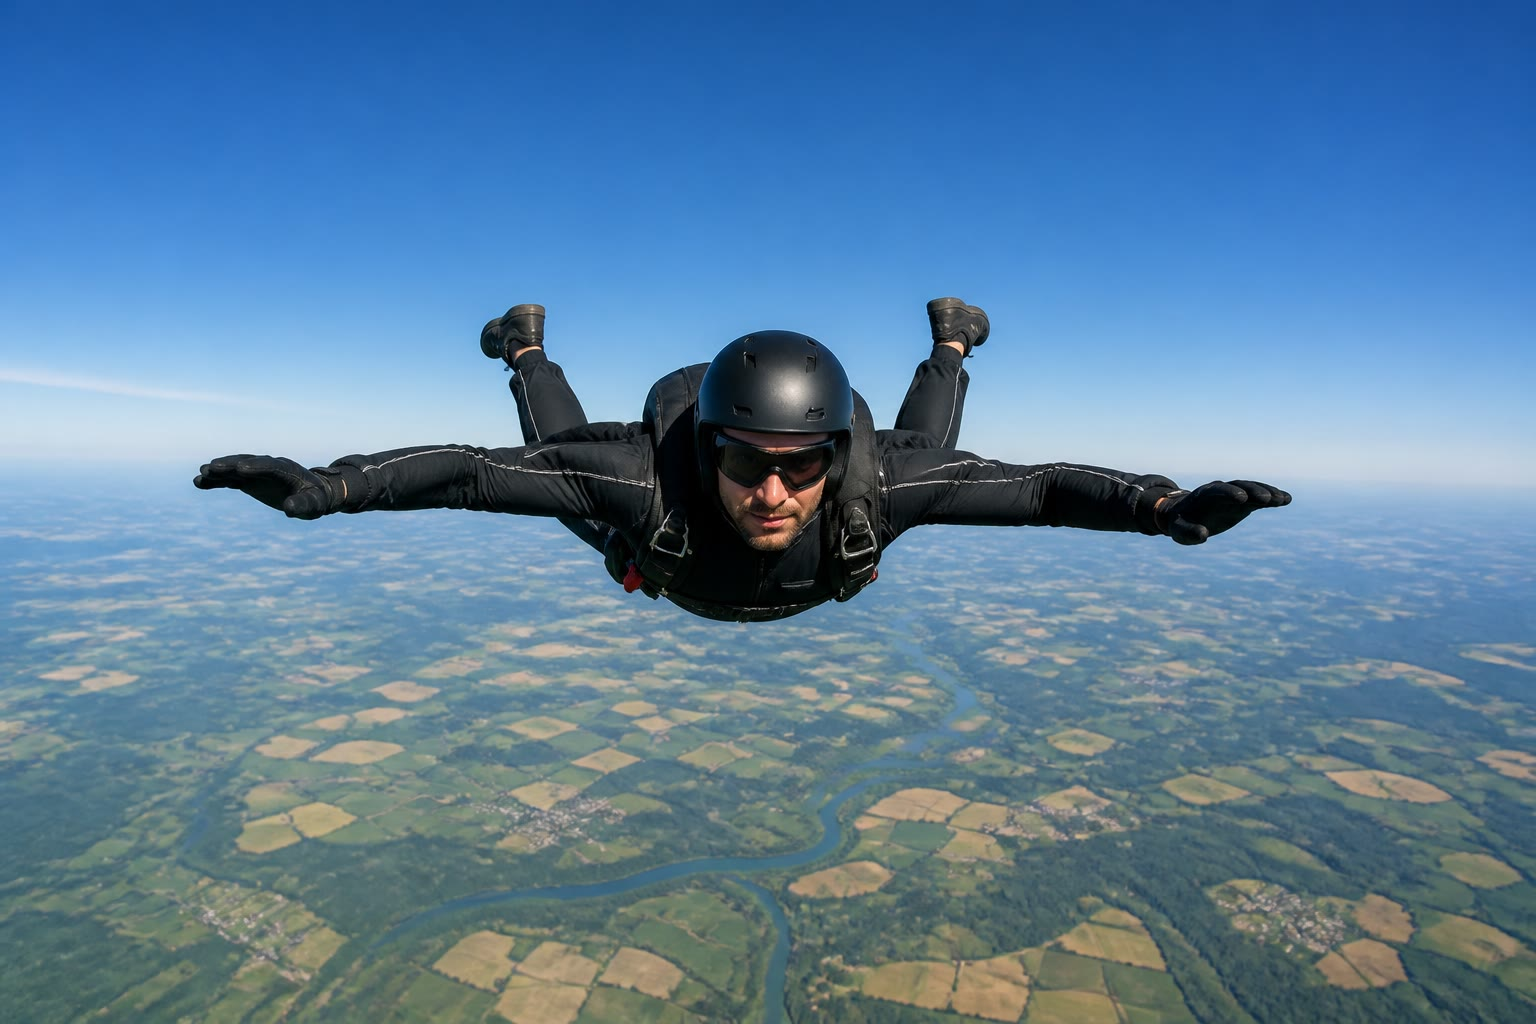
\includegraphics[width=0.60\linewidth]{images/book3/ai/b3-12-skydiver-freefall.jpg}

{\small 有空气时的自由下落：数秒之后，二次阻力与重力平衡，跳伞者以接近 \qty{200}{km/h} 的终端速率下落——即周末问题。}
\end{omfigure}

\section{周末问题：跳伞者}

\begin{problem}[{周末问题——从机舱门到
地面：自由下落、空气阻力、开伞过快的降落伞，
以及着陆——一条运动定律，两种阻力定律}]
\label{pb:b1:newton-dynamics:1}
装备齐全的跳伞者质量为 $m = \qty{80}{kg}$。空气：
$\rho = \qty{1.2}{kg/m^3}$，$\eta = \qty{1.8e-5}{Pa.s}$。俯身下落时，
$C_xS = \qty{0.80}{m^2}$；张伞后，$C_xS =
\qty{25}{m^2}$。$g = \qty{9.81}{m/s^2}$；$z$ 竖直向下为正，
从跳伞点起算。

\medskip
\noindent\textbf{第一部分——无空气情形。}
\begin{enumerate}
  \item 写出牛顿第二定律，并给出 $v(t)$ 和 $z(t)$；计算
        两者在 $t = \qty{10}{s}$ 时的值。
  \item 计算重力。
  \item 在此阶段，跳伞者感到“失重”，尽管
        重力仍完全作用。请用受力解释（与站在地面上相比，
        缺了什么力）。
  \item 对于本题，地球参考系是否足够近似为惯性参考系？请指出
        被忽略的是什么。
\end{enumerate}

\medskip
\noindent\textbf{第二部分——在空气中下落。}
\begin{enumerate}[resume]
  \item 写出俯卧下落时阻力关于 $v$ 的表达式。
  \item 写出 $v(t)$ 所满足的运动方程。
  \item 求终端速度 $v_\infty$（分别以 \unit{m/s} 和
        \unit{km/h} 表示）。
  \item 令 $u = v/v_\infty$，$\tau = v_\infty/g$，证明
        $\dd u/\dd t = (1 - u^2)/\tau$；计算 $\tau$。
  \item 用分离变量法求解，并证明
        $v = v_\infty\tanh(t/\tau)$。
  \item 经过多长时间 $v = 0.9v_\infty$？$0.99v_\infty$？
  \item 证明 $z(t) = v_\infty\tau\ln\cosh(t/\tau)$，并计算
        $t = \qty{10}{s}$ 时下落的距离；并与第一部分作比较。
  \item 估算 $v_\infty$ 处的雷诺数，取 $L = \qty{0.5}{m}$，
        并说明二次定律的合理性。
\end{enumerate}

\medskip
\noindent\textbf{第三部分——降落伞张开。}
\begin{enumerate}[resume]
  \item 计算伞张开后的新终端速度。
  \item 若伞在 $v = \qty{40}{m/s}$ 时瞬间张开，
        减速度将为多少，以 \unit{m/s^2} 和 $g$ 表示？
        为什么这是不可接受的？
  \item 实际的伞需要约 \qty{3}{s} 才能张开。估算
        平均减速度，以及背带对跳伞者的
        平均作用力。
  \item 伞完全张开后，速率将趋向新的
        $v_\infty$：求新的时间常数 $\tau' = v_\infty'/g$，
        以及这对趋于稳定下降意味着什么？
  \item 稳定下降时，背带的作用力是多少？用
        第二定律加以说明。
  \item 解释终端速度为何与 $1/\sqrt{C_xS}$ 成正比。若伞面积
        减半，终端速度将提高为原来的多少倍？
  \item 一位较重的跳伞者（\qty{100}{kg}）使用同一顶伞，其
        终端速度为多少？
\end{enumerate}

\medskip
\noindent\textbf{第四部分——着陆。}
\begin{enumerate}[resume]
  \item 着地速度即伞的 $v_\infty$。若不计空气，
        则需从多高处跳下，才能以该速度
        触及地面？
  \item 双腿僵直着地时，身体在 \qty{0.5}{m} 内停止；翻滚着地
        时则在 \qty{1.5}{m} 内停止。估算平均减速度（以 $g$ 表示）
        以及两种情形下腿部所受的平均作用力，并作出结论。
  \item 在即将触地前，跳伞者同时拉下两根拉绳，
        这会暂时增大伞的阻力。定性解释
        这对速率的影响。
\end{enumerate}

\medskip
\noindent\textbf{第五部分——小物体的下落方式不同。}
\begin{enumerate}[resume]
  \item 一个半径为 \qty{1.0}{mm}（$C_x = 0.5$）的雨滴：用二次定律计算其
        终端速度，并检验
        雷诺数。
  \item 一个半径为 \qty{10}{\micro m} 的雾滴：用斯托克斯定律求
        $v_\infty$，并检验雷诺数
        确实很小。
  \item 总结：一个运动方程，两种阻力区域，以及
        决定某物是像石头一样下落、像树叶一样飘落，
        还是根本不落的三个数值（\unit{m/s}）。
\end{enumerate}
\end{problem}
